\documentclass{article} % For LaTeX2e
\usepackage{iclr2022_conference,times}
\usepackage{graphicx}
\usepackage{booktabs}
\usepackage{multirow}
\usepackage{amsmath}
% Optional math commands from https://github.com/goodfeli/dlbook_notation.
\input{math_commands.tex}

%######## APS360: Uncomment your submission name
%\newcommand{\apsname}{Project Proposal}
\newcommand{\apsname}{Progress Report}
%\newcommand{\apsname}{Final Report}

%######## APS360: Put your Group Number here
\newcommand{\gpnumber}{42}

\usepackage{hyperref}
\usepackage{url}
\usepackage{graphicx}
\usepackage{tabularx}
\usepackage{geometry}


%######## APS360: Put your project Title here
\title{PROJECT TITLE}


%######## APS360: Put your names, student IDs and Emails here
\author{Vedansh Mehta  \\
Student\# 1008973577 \\
\texttt{vedansh.mehta@mail.utoronto.ca} \\
\And
Nathan Shreve  \\
Student\# 1004404487 \\
\texttt{n.shreve@mail.utoronto.ca} \\
\AND
William Wen  \\
Student\# 1007956650 \\
\texttt{jwilliam.wen@mail.utoronto.ca} \\
\And
Paul Zhao \\
Student\# 1009052276 \\
\texttt{paul.zhao@mail.utoronto.ca} \\
\AND
}

% The \author macro works with any number of authors. There are two commands
% used to separate the names and addresses of multiple authors: \And and \AND.
%
% Using \And between authors leaves it to \LaTeX{} to determine where to break
% the lines. Using \AND forces a linebreak at that point. So, if \LaTeX{}
% puts 3 of 4 authors names on the first line, and the last on the second
% line, try using \AND instead of \And before the third author name.

\newcommand{\fix}{\marginpar{FIX}}
\newcommand{\new}{\marginpar{NEW}}

\iclrfinalcopy 
%######## APS360: Document starts here
\begin{document}


\maketitle

\begin{abstract}
    % ABSTRACT HERE
    %######## APS360: Do not change the next line. This shows your Main body page count.
    This report details the progress on developing a deep learning model for detecting AI-generated images. The model is constructed with a two-step approach which involves separately training a convolutional autoencoder (CAE), which learns real image statistics, and a classifier that differentiates real and synthetic images based on reconstruction loss from the CAE. The team utilized the Chameleon dataset \citep{yan2024sanity}, which includes semantically balanced real and AI-generated images to train and test the model. This dataset was split into two sets for CAE training and classifier training, respectively, before preprocessing, wherein the images were resized and normalized. At the moment we have trained three models: a baseline model, which achieves an accuracy of 65.6\%, our primary model (as described above), which currently performs randomly, and a backup model, which achieves an accuracy of 89.2\%. Future steps on the primary model include hyperparameter tuning, incorporating transfer learning, and training on additional datasets.
    ----Total Pages: \pageref{last_page}
\end{abstract}



\section{Project Description}
\label{project_description}

The rise of hyper-realistic AI-generated images, from deepfake scams SOURCE to synthetic propaganda SOURCE, has eroded digital trust SOURCE. Our project, a classifier which distinguishes between real and AI-generated images, addresses this issue. We aim to create a zero-shot model that works on images generated by any image synthesis model, eliminating the need for updates as new models arise. This model can be used by journalists to verify photos, by social media platforms to block harmful content, and by internet users who want to avoid mis- and disinformation.


Traditional methods, such as spectral analysis, fail at identifying AI-generated images because they cannot generalize across various architectures such as DALL-E and Stable Diffusion SOURCE. A deep learning model is needed to identify the outputs of other deep learning models. Our method, illustrated in FIGURE X, involves two steps: first, we train a CAE on real images, so that it reconstructs real images well and AI-generated images badly. Next, we freeze the CAE, pass both real and AI-generated images through it, and use pixel-wise loss to delineate the two classes. Since our CAE is trained only on real images, it does not need to be retrained upon the advent of new image synthesis architectures and models.


\section{Individual Contributions and Responsibilities}

The team holds weekly meetings every Sunday at 10 a.m. online using Zoom to discuss the project progress, direction, and task distribution. The meeting time is tentatively changed every week depending on team member availability. In case of a need for a time change, the new meeting time is discussed and communicated on or before the Friday of the week. The team utilizes WhatsApp for daily communication, small updates, and any questions regarding the project or the course. Under circumstances where additional meetings need to be arranged, a member will send a WhatsApp message and it is expected that all team members will react to the message in less than 12 hours.

To maintain a convenient and clean working environment, we store all code, documents, and research apart from our data in our GitHub repository. Code development is managed through a Google Colab Notebook with three sections: Data Processing, Baseline Model, and Primary Model. Written documents are done in \LaTeX{}. The GitHub repository includes a Wiki which allows us to track our progress. Each Wiki page contains a table of assigned tasks, internal deadlines, hard deadlines, assignees, and task statuses. All team members are expected to regularly update this table.

Under the circumstance where a team member cannot meet the internal deadline for a certain task, they shall notify the rest of the team through WhatsApp. Tasks will be reassigned either through WhatsApp communication or during a Zoom meeting.

Table \ref{Progress_Report_Task_Distribution} details our current task distributions, including deadlines and completion statuses, for the Progress Report and the project itself.

\begin{table}[htp]
    \caption{Progress Report Task Distribution}
    \label{Progress_Report_Task_Distribution}
    \begin{center}
        \begin{tabular}{|>{\raggedright\arraybackslash}p{4cm}|>{\raggedright\arraybackslash}p{2.5cm}|>{\raggedright\arraybackslash}p{2cm}|>{\raggedright\arraybackslash}p{2cm}|>{\raggedright\arraybackslash}p{1.5cm}|}
            \hline
            \textbf{Task}                                                                                     & \textbf{Assignee(s)} & \textbf{Internal Deadline} & \textbf{Hard Deadline} & \textbf{Status} \\
            \hline
            Split Data For Two Step Training Process                                                          & William              & Mar. 02, 2025              & Mar. 06, 2025          & completed       \\
            \hline
            Build, train, test and debug baseline model                                                       & Nathan \& William    & Mar. 03, 2025              & Mar. 06, 2025          & completed       \\
            \hline
            Research on Convolutional Auto-encoder Architecture                                               & William              & Mar. 03, 2025              & Mar. 06, 2025          & completed       \\
            \hline
            Build, train, test, and debug step 1 of primary model                                             & Nathan \& William    & Mar. 04, 2025              & Mar. 06, 2025          & completed       \\
            \hline
            Research on existing models that could be applied for Transfer Learning                           & Paul \& Vedansh      & Mar. 05, 2025              & Mar. 06, 2025          & completed       \\
            \hline
            Research on visualization software                                                                & William              & Mar. 06, 2025              & Mar. 06, 2025          & completed       \\
            \hline
            Research on compression defects removal                                                           & William              & Mar. 06, 2025              & Mar. 06, 2025          & completed       \\
            \hline
            Write Introduction of Progress Report                                                             & Vedansh              & Mar. 06, 2025              & Mar. 06, 2025          & completed       \\
            \hline
            Write Individual Contributions and Responsibilities for Progress Report                           & Paul                 & Mar. 06, 2025              & Mar. 06, 2025          & completed       \\
            \hline
            Write Data Processing in Notable Contribution for Progress Report                                 & William              & Mar. 06, 2025              & Mar. 06, 2025          & completed       \\
            \hline
            Write Baseline Model and Primary Model in Notable Contribution for Progress Report                & Nathan               & Mar. 06, 2025              & Mar. 06, 2025          & completed       \\
            \hline
            Research on Optuna - an automated hyperparameter search tool. Apply it to CAE                     & Paul                 & Mar. 15, 2025              & Mar. 20, 2025          & on-going        \\
            \hline
            Research on more architectures using Resnet. Potentially implement a stronger Resnet architecture & Vedansh \& Paul      & Mar. 20, 2025              & Mar. 25, 2025          & on-going        \\
            \hline
            Reprocess and regroup real images from Chameleon to enhance autoencoder learning                  & William              & Mar. 20, 2025              & Mar. 25, 2025          & on-going        \\
            \hline
            Explore more architecture configurations for classifier                                           & Nathan               & Mar. 20, 2025              & Mar. 25, 2025          & on-going        \\
            \hline
        \end{tabular}
    \end{center}
\end{table}



\section{Notable Contributions}
\subsection{Data Processing}

For data processing, we implemented a two-step approach. The first step splits the data and saves it into properly structured folders for easy extraction later. The second step uses PyTorch built-in classes to preprocess images.
\subsubsection{Source of Dataset}
The dataset for our project, named the \textbf{Chameleon Dataset}, was obtained from \emph{A Sanity Check for AI-Generated Image Detection}, published at ICLR 2025 \citep{yan2024sanity}. We selected this dataset for two main reasons:

\begin{itemize}
    \item It contains a balanced collection of real and AI-generated images across multiple categories, including humans, animals, objects, and scenes.
    \item Unlike datasets such as AIGCDetect \citep{rptc} and GenImage \citep{zhu2023gendet}, which contain raw AI-generated images with visible defects, the AI-generated images in the Chameleon dataset are carefully refined by photographers and AI artists. These high-quality images have been shown to fool nine off-the-shelf AI-generated image detectors \citep{yan2024sanity}.
\end{itemize}

% \begin{figure}[h]
%     \centering
%     \includegraphics[width=1\textwidth]{figs/Chameleon.jpg}
%     \caption{Comparison between AIGCDDetect (a) and GenImage (b) with Chameleon Dataset(c) \citep{yan2024sanity}.}
%     \label{fig:Chameleon}
% \end{figure}

Given our goal of detecting general AI-generated images (both raw and adjusted), training our model on this challenging dataset should enable it to generalize well.

\subsubsection{Data Splitting}

To prepare our dataset for our two-step architecture in Section \ref{primary_model}, we implemented the following steps:
\begin{enumerate}
    \item Load the Chameleon dataset (ZIP file) from Google Drive.
    \item Unzip the file and extract image paths from the \texttt{01\_real} and \texttt{02\_fake} subfolders.
    \item Shuffle the images to ensure randomness in splitting.
    \item Identify the total number of real images: 14,863.
    \item Split the real images into two halves: 7,431 for step 1 (CAE) and 7,432 for step 2 (classifier).
    \item Randomly select the same number of fake images (7,432) to ensure a balanced dataset for step 2.
    \item Split the dataset into train, validation, and test sets with a 75/20/5 ratio.
    \item Store the images in structured directories on a shared Google Drive.
\end{enumerate}

The folder structure and number of samples in each class for the two steps is shown in Figure \ref{fig:cleaned_statistic}.

\begin{figure}[h]
    \begin{center}
        \includegraphics[scale=0.5]{figs/cleaned_statistic.png}
    \end{center}
    \caption{Processed data statistics.}
    \label{fig:cleaned_statistic}
\end{figure}

\subsubsection{Data Processing and Augmentation}
The processing step occurs when loading the data using \texttt{ImageFolder} and \texttt{Transforms}. The current preprocessing pipeline involves randomly resizing images to 256×256 through cropping, converting them to tensors, and normalizing them into the range [$-1$, $1$]. Some examples are shown in Figure \ref{fig:cleaned_sample}.

\begin{figure}[h]
    \begin{center}
        \includegraphics[width=0.6\textwidth]{figs/data_examples_2by3.png}
    \end{center}
    \caption{Examples of four cleaned samples from the dataset.}
    \label{fig:cleaned_sample}
\end{figure}

No data augmentation has been applied yet. However, we are considering methods such as flipping, and color jittering, which may be implemented depending on the training results.

We deliberately chose not to perform compression artifact removal, as we believe this might remove original defects from AI-generated images that might serve as distinguishing features. However, we have considered tools for compression defect removal, such as Hi-IR \citep{li2024hierarchicalinformationflowgeneralized}.

Examples of processed images are shown in Figure \ref{fig:cleaned_sample}.


\subsubsection{Future Test Set}
While we have set aside 5\% of the dataset for testing on each step, we still need an external test set to evaluate the model on never-before-seen data as a final step. To achieve this, we plan to
collect 100 real-world images from personal sources, covering humans, animals, objects, and scenes and generate 100 AI-generated images using state-of-the-art generators such as DALL-E, MidJourney, and Stable Diffusion.

\subsubsection{Challenges}
One of the challenges we encountered was uploading the Chameleon Dataset, which is approximately 2.7 GB in size. Initially, this process was time-consuming when using a direct upload to Google Drive. To address this, we opted to upload the dataset as a ZIP file and extract it directly within PyTorch, significantly reducing transfer times.

\subsection{Baseline Model}

\begin{figure}[h]
    \begin{center}
        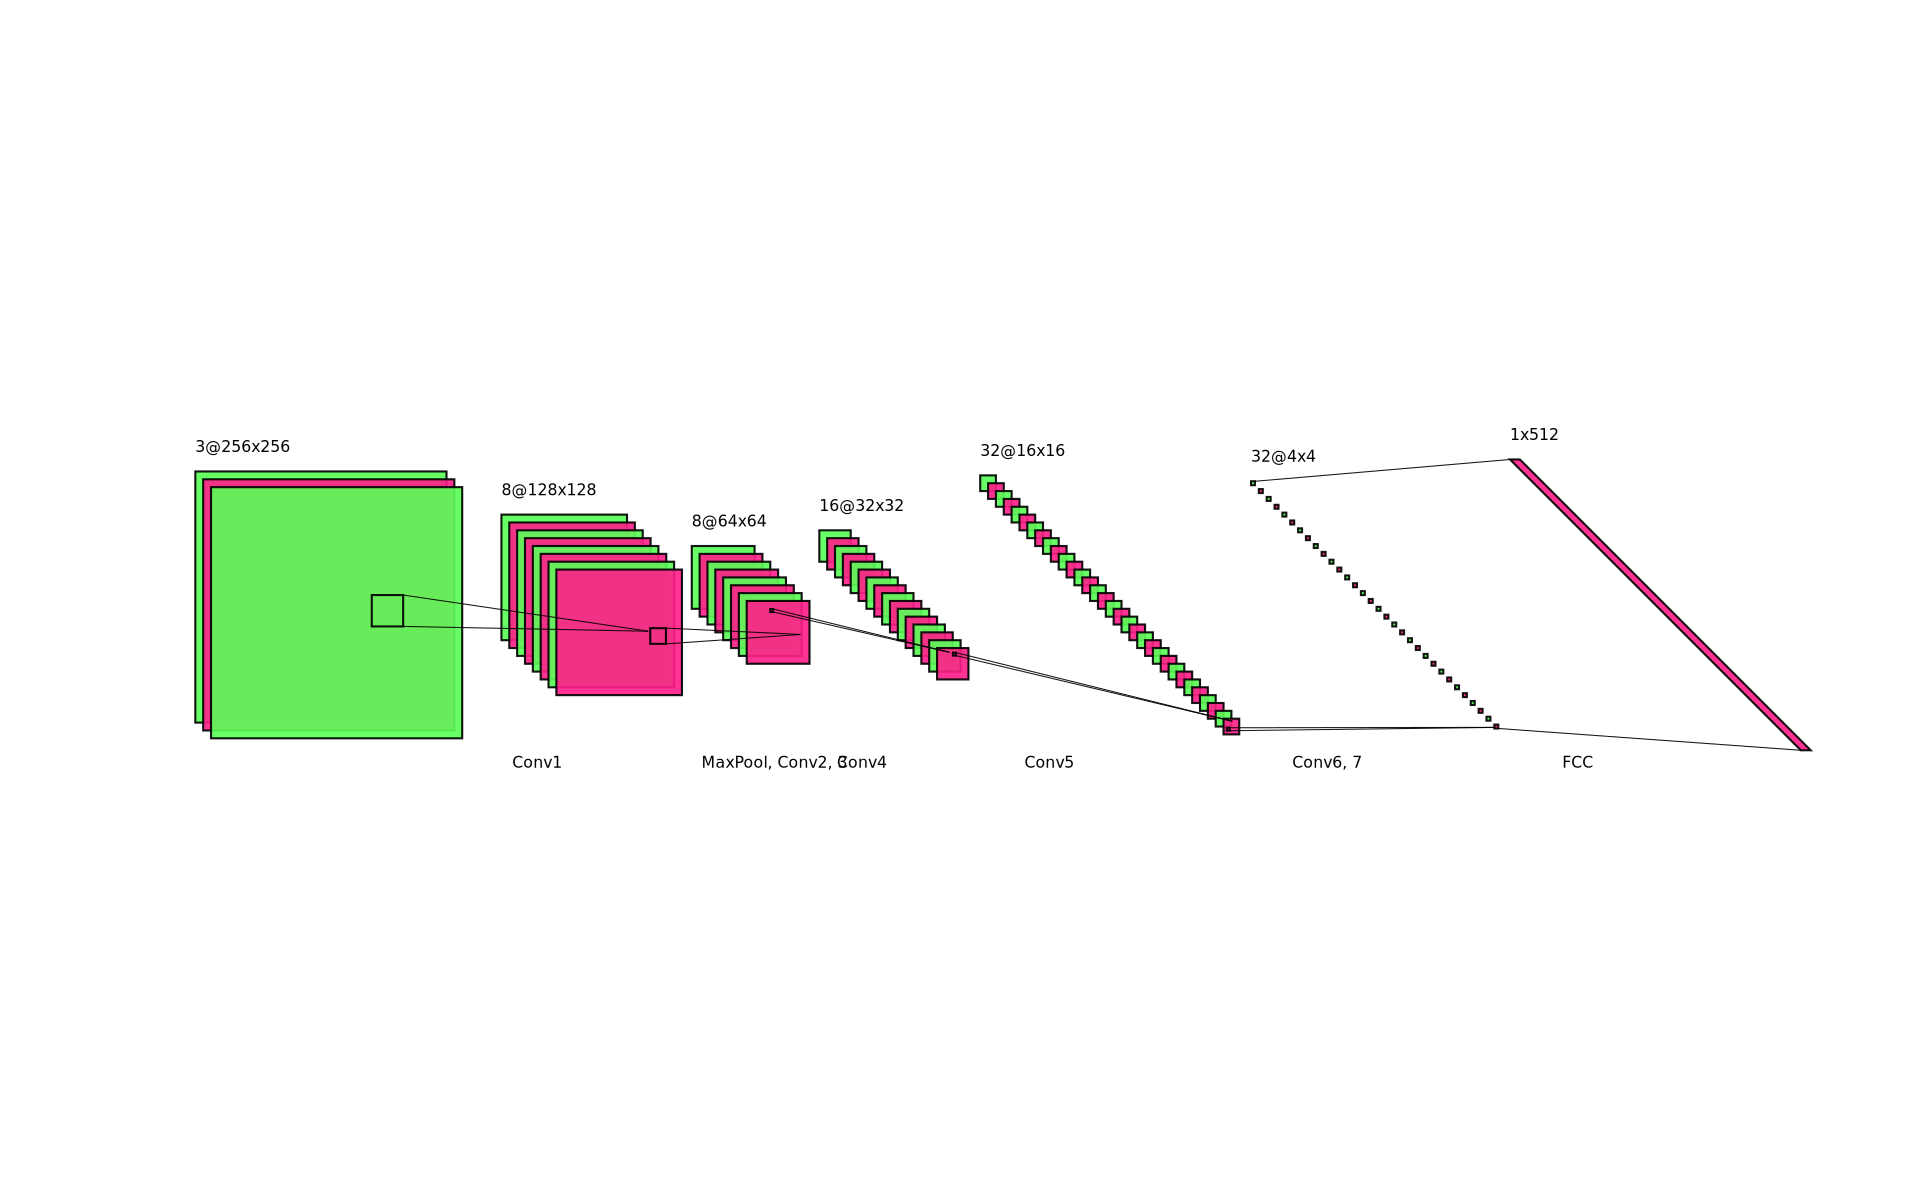
\includegraphics[scale=0.45]{figs/baseline.png}
    \end{center}
    \caption{Baseline model architecture, simplified; the final fully connected layer to a single output neuron.}
    \label{fig:baseline_arch}
\end{figure}

As outlined in the Project Proposal, we wrote a CNN inspired by \citet{wang2020cnngeneratedimagessurprisinglyeasy}, which is roughly illustrated in Figure \ref{fig:baseline_arch}. It has seven convolutional layers and a total of $1,195,009$ parameters. Between each layer, we applied ReLU and batch normalization. We used a batch size of 64, a learning rate of 0.01, stochastic gradient descent (SGD) with momentum 0.9, and a binary cross-entropy loss function. We wanted to train over $3,000$ iterations, which corresponded to 17 epochs.

We observed that, across various hyperparameter combinations, validation curves were quite jagged, though they declined with the training curve (see Figure \ref{fig:baseline_curves}). The model learns the training data slowly, yet struggles to generalize. This is most likely due to the complex nature of the task, which demands greater parameters and epochs than ours. In our best model we were able to achieve a validation accuracy of 67.0\% and a testing accuracy of 65.6\%. Detailed classification statistics for each split can be seen in Table \ref{baseline_stats}.

\begin{table}[t]
    \caption{Baseline model error statistics; real images are negatives and AI-generated images are positives.}
    \label{baseline_stats}
    \begin{center}
        \begin{tabular}{llllll}
            \multicolumn{1}{c}{\bf Split} & \multicolumn{1}{c}{\bf Loss} & \multicolumn{1}{c}{\bf Accuracy} & \multicolumn{1}{c}{\bf Precision} & \multicolumn{1}{c}{\bf Recall} & \multicolumn{1}{c}{\bf F1 Score}
            \\ \hline \\
            Training                      & 0.303                        & 87.3\%                           & 85.8\%                            & 89.5\%                         & 87.6\%                           \\
            Validation                    & 0.947                        & 67.0\%                           & 66.2\%                            & 69.6\%                         & 67.8\%                           \\
            Testing                       & 0.919                        & 65.6\%                           & 64.7\%                            & 68.5\%                         & 66.6\%                           \\
        \end{tabular}
    \end{center}
\end{table}

\begin{figure}[h]
    \begin{center}
        \includegraphics[scale=0.45]{figs/baseline_error_curves.png}
        \includegraphics[scale=0.45]{figs/baseline_loss_curves.png}
    \end{center}
    \caption{Training/validation error (left) and loss (right) curves for the best baseline model.}
    \label{fig:baseline_curves}
\end{figure}

\subsection{Primary Model}
\label{primary_model}

As outlined in Section \ref{project_description}, we are using a two-step anomaly detection approach. In the first step, we trained a CAE to encode and decode real images only. In the second step, we feed both real and AI-generated images into the CAE, compute pixel-wise loss, and give this loss to a CNN which classifies the image as real or AI-generated. The advantage of this two-step strategy is that the first is zero-shot, and would not require retraining upon the advent of new image synthesis models. However, we have struggled with this approach, and propose new ideas in Section \ref{next_steps}.

\subsubsection{Convolutional Autoencoder}

The purpose of our CAE is to model real images well, so it was trained only on real images. It uses up to seven convolutional layers for the encoder and decoder each, with up to $1,970,755$ parameters. We experimented with 30 different combinations of various hyperparameters, including our activation function, number of encoder/decoder layers, weight initialization, batch size, learning rate, optimizer, and loss function.

Our main challenge in training using the Adam optimizer effectively. Early on, we used a learning rate of 0.01, but we observed that the Adam optimizer was extremely ineffective and could not generalize: validation curves oscillated without decreasing. We then attempted to use a learning rate of 0.0001, and the validation loss greatly decreased in early epochs before overfitting, and outperformed SGD.

Our best model used LeakyReLU, no weight initialization, a batch size of 64, a learning rate of $0.0001$, the Adam optimizer with weight decay of $0.01$, and MSE loss. We also used six encoder/decoder layers, which correspond to a compression ratio of 48. Though this model overfit early during training (see Figure \ref{fig:cae_curves}), we were not able to achieve a lower validation loss before overfitting occurred when using lower learning rates. This model achieves a validation MSE of 0.084 and a test MSE of 0.083, which correspond to about 14.4\% absolute error per pixel.

\begin{figure}[h]
    \begin{center}
        \includegraphics[width=0.45\textwidth]{figs/cae_error_curves.png}
    \end{center}
    \caption{Training/validation error curves for the best CAE.}
    \label{fig:cae_curves}
\end{figure}

As mentioned earlier, we want the CAE to model real images well and to model AI-generated images badly. Therefore, we also evaluated this model on a separate test set containing both real and AI-generated images with the expectation that the error would be much higher. However, it was also $0.083$, suggesting that our CAE has not learned the characteristics that comprise real images, but rather the semantic content of our dataset and, possibly, patterns produced by the images' compression. The output of the CAE for one real and one AI-generated image is shown in Figure \ref{fig:reconstructions}. We can see that it reconstructs both with an equal lack of detail, suggesting it has not really learned a good representation of real images.

\begin{figure}[h]
    \begin{center}
        \includegraphics[scale=0.25]{figs/reconstructions.png}
    \end{center}
    \caption{Best autoencoder's reconstructions of real (top) and AI-generated (bottom) faces.}
    \label{fig:reconstructions}
\end{figure}

\subsubsection{Classifier}

The input to our classifier is the pixel-wise CAE reconstruction loss at the output of our CAE. We have experimented with a number of reconstruction loss functions, such as MSE, L1 loss, and Huber loss.

This step is still in early development. At the moment, our classifier uses the same architecture as our baseline model, but without skip connections. However, we have not been able to achieve much better than random results. As mentioned earlier, this is most likely because our CAE models real and fake images equally well.
\subsection{Transfer Learning: ResNet}
\label{transfer_learning}

Due to our struggles with developing a zero-shot model, we have begun developing a ``backup'' model to ensure project success. This model is a classifier which uses a pretrained ResNet18 trained on ImageNet with frozen convolutional layers. At the output of these convolutional layers, we trained a 512-unit fully connected layer which feeds into a single output neuron. This hidden layer uses ReLU activation and dropout with $p=0.5$. We used binary cross-entropy loss, the Adam optimizer, and trained for 25 epochs.

As shown in Figure \ref{fig:transfer_curves}, the model achieved much greater success than our baseline and primary models: 88.8\% validation accuracy and a corresponding 89.2\% test accuracy. We have not begun tuning hyperparameters (we have only trained the model once) and have only observed minimal overfitting, so there is room to improve this result.

\begin{figure}[h]
    \begin{center}
        \includegraphics[width=0.95\textwidth]{figs/transfer learning graphs.jpg}
    \end{center}
    \caption{Training and validation loss and accuracy curves for the ResNet18-based model.}
    \label{fig:transfer_curves}
\end{figure}

\subsection{Next Steps}
\label{next_steps}

Below are a number of new ideas we will implement that address our struggles outlined above.

\begin{itemize}
    \item[1.] Use transfer learning, such as ResNet: pass our images through a pretrained model, and pass the output either into our autoencoder or directly to a decoder.
    \item[2.] Use transfer learning to classify our images into a small number of classes based on semantic content (around 10), then train an autoencoder for each class.
    \item[3.] Find new data, in particular images that are uncompressed, to either supplement or supplant our current dataset.
    \item[4.] Continue to develop and tune the model described in Section \ref{transfer_learning}.
\end{itemize}

\label{last_page}

\bibliography{APS360_ref}
\bibliographystyle{iclr2022_conference}

\end{document}
